\documentclass[12pt,oneside]{book}
\usepackage[utf8]{inputenc}
\usepackage{amsmath, amsfonts, amssymb}

\usepackage{enumitem} % to control the manual enumerations dynamically

\usepackage{multirow}
\usepackage{multicol}
\usepackage{longtable}
\usepackage{booktabs}
\usepackage{needspace} %to make sure that no pagebreaks in certain situations
\usepackage{setspace}
\usepackage{blindtext}
%%%%%%%------------------------------------------------
%%%%%%-----------Page Layout Setups------
%%%%%%--------------------------------------------------
\usepackage{geometry}
\geometry{
	headheight=6ex,
	includehead,
	includefoot
}
\geometry{
	paper=a4paper,% Change to letterpaper for US letter
	inner=1in, % Inner margin
	outer=1in, % Outer margin
	bindingoffset=1cm, % Binding offset
	top=1in, % Top margin
	bottom=1in, % Bottom margin
	%showframe,% show how the type block is set on the page
}
\renewcommand{\baselinestretch}{1.3} % for line spacing
\usepackage{fancyhdr}%for the header and footer
\usepackage{emptypage}%to remove headers and footers in the blank pages	

\pagestyle{fancy} %Initiates the Page Style

\fancyhf{}
\renewcommand{\headrulewidth}{1pt}
%\fancyhead[L]{\nouppercase \leftmark}
\fancyhead[R]{\nouppercase \rightmark}
\renewcommand{\footrulewidth}{0.7pt}
\fancyfoot[L]{\small \em \printtitle}
\fancyfoot[R]{\thepage}




%%%%%%-----------------------------------------------
%%%%%%------------ Font Set up --------------
%%%%%%-----------------------------------------------
%\usepackage{fouriernc}
%\usepackage{newtxtext,newtxmath}
%\usepackage[T1]{fontenc} 
%\usepackage{mathdesign}
%\usepackage{mathptmx}
%\usepackage{utopia}
\usepackage{times} %Use this for Times New Roman
%\usepackage{helvet}
%\usepackage{lmodern}

%%%%%%------------------------------------------------
% % % %-----------------For the graphics-------
%%%%%%------------------------------------------------
\usepackage{graphicx}
\usepackage{subcaption}
\graphicspath{{./images/}}
\usepackage[usenames,dvipsnames,svgnames,table]{xcolor} % for colors
\usepackage{float}
\usepackage{tikz}
\usepackage[many,breakable]{tcolorbox}

%%%% Highlighter-----------------------------------------------
\makeatletter
\newcommand{\hl}[1]{%
	\setbox\@tempboxa\hbox{#1}%
	\ifdim\wd\@tempboxa>\linewidth
	\noindent
	\colorbox{pink}{%
		\parbox{\dimexpr\linewidth-2\fboxsep}{#1}%
	}%
	\else
	\colorbox{pink}{#1}%
	\fi}%Highlighter.
\makeatother
% % % % % % % %---------------------------------------
% % % % % % % %-------BibLatex------------------------
% % % % % % % %---------------------------------------
\usepackage[backend=bibtex,maxbibnames=6,defernumbers=true,natbib=true, sorting=none,  style = ieee,  url = false, doi = false]{biblatex}
\addbibresource{main.bib}



%%%%%------------------------------------------------
%%%%%-----------Hyperlinks Setup---------------------
%%%%%------------------------------------------------

\usepackage{hyperref}
\hypersetup{
	colorlinks=true,
	linkcolor=sec,
	filecolor=red,      
	urlcolor=sec,
	citecolor = sec
}

%%%%%------------------------------------------------
%%%%%-----------Title format-------------------------
%%%%%------------------------------------------------

\usepackage{etoolbox}
%\makeatletter
%\patchcmd{\chapter}{\if@openright\cleardoublepage\else\clearpage\fi}{}{}{}
%\makeatother

\newcommand{\Hrule}{\rule{\linewidth}{1mm}}



\usepackage[explicit]{titlesec}
\usepackage[titletoc]{appendix}
\definecolor{sec}{HTML}{154360}
\definecolor{band}{HTML}{EE9C52}


\makeatletter
\newcommand{\setappendix}{Appendix~\thechapter}
\newcommand{\setchapter}{Chapter~\thechapter~} 
\titleformat{\chapter}[display]{\sffamily\bfseries \huge\color{sec}}{}{0.5ex} %
{\ifnum\pdfstrcmp{\@currenvir}{appendices}=0
	\setappendix
	\else
	\setchapter
	\fi 
	\filleft \\%
	\titlerule[1pt]
	\vspace{1ex}%
#1\filleft\\
	\vspace{1ex}%
	\titlerule[3pt]}

\titleformat{name=\chapter, numberless}[display]{ \color{sec}\sffamily\bfseries\huge}{ }{0.5ex} %
{ \titlerule[1pt]
	\vspace{1ex}%
	#1\filleft
	\addcontentsline{toc}{chapter}{#1}
	\markboth{}{#1}\\
	\vspace{1ex}%
	\titlerule[3pt]}
\makeatother

\titlespacing*{\chapter}{0ex}{-10ex}{0ex}

\titleformat{\section}{\Large\bfseries}{}{0.0ex} %
{\sffamily\color{sec} \thesection~#1 \filright}[\smallskip]

\titleformat{name = \section, numberless}{\Large\bfseries}{}{0.0ex}%
{\sffamily\color{sec}#1\filright}[\smallskip]

\titleformat{\subsection}[hang]{\sffamily\Large\bfseries}{}{0.5ex}%
{\color{sec}\thesubsection~#1\filright}[\smallskip]

\titleformat{name = \subsection, numberless}[hang] {\sffamily\Large\bfseries}{}{0.5ex}%
{\color{sec}#1\filright}[\smallskip] 



%%%%%%%%%---------------------------------------------	
%%%%%%%%%----------New Theorems & Environments-------------------
%%%%%%%%%---------------------------------------------
\usepackage{amsthm}
\usepackage{thmtools} % handles autoref efficiently
\newtheorem{theorem}{Theorem}[chapter]  
\newtheorem{lemma}[theorem]{Lemma}%[section]
\newtheorem{corollary}[theorem]{Corollary}%[section]
\newtheorem{proposition}[theorem]{Proposition}%[section]




\theoremstyle{definition}
\newtheorem{question}{Question}
\newtheorem{conjecture}{Conjecture}
\newtheorem{example}[theorem]{Example}
\newtheorem{recall}{Recall}
\newtheorem{remark}[theorem]{Remark}
\newtheorem{definition}[theorem]{Definition}


\numberwithin{equation}{chapter}
\numberwithin{figure}{chapter}
\numberwithin{table}{chapter}


\newenvironment{keywords}{\noindent\textbf{Keywords:}}{}
\newenvironment{classification}{\noindent\textbf{AMS subject classifications:}}{}
%%%%%%%%%----------------------------------------------	
%%%%%%%%%----------for the Abstract environment:-------
%%%%%%%%%----------------------------------------------
\newcommand\abstractname{Abstract}  %%% here
\makeatletter
\newenvironment{abstract}{%
	\if@twocolumn
	\section*{\abstractname}%
	\else
	\small
	\begin{center}%
		{\bfseries \abstractname\vspace{-.5em}}%
	\end{center}%
	\quotation
	\fi}
{\if@twocolumn\else\endquotation\fi}
%	\fi
\makeatother
%	\listfiles %%To check the versions of the packages used

%----------------------------------------------------------------------------------------
%	PENALTIES( for the Hypenation Problem)
%----------------------------------------------------------------------------------------

\doublehyphendemerits=10000 % No consecutive line hyphens
\brokenpenalty=10000 % No broken words across columns/pages
\widowpenalty=9999 % Almost no widows at bottom of page
\clubpenalty=9999 % Almost no orphans at top of page
\interfootnotelinepenalty=9999 % Almost never break footnotes

%-----------------------------------------------------
%%Rulers used in Title page and other pages-----------
%-----------------------------------------------------
\newcommand{\decoRule}{\rule{.8\textwidth}{.4pt}}
\newcommand{\HRule}{\rule{\linewidth}{0.5mm}}

%%%% -----------------------------------------------------
%%%%--------- Index ---------------------------------
%%%% -----------------------------------------------------
\usepackage{imakeidx}
\makeindex[title={Subject Index},columns=1]
\makeindex[name=a,title=\uppercase{Author Index},columns=2]
\usepackage[font=small]{idxlayout}

\makeatletter
\newcommand\thesistitle[1]{\renewcommand\@thesistitle{#1}}
\newcommand\@thesistitle{} % To keep default empty
\newcommand{\printtitle}{\makeatletter \@thesistitle \makeatother} %to print the title wherever you need
\makeatother



\newcommand\dedicatory[1]{
	\clearpage 
	\null\vfil
	\thispagestyle{empty}
	\begin{center}{\Large\slshape #1}\end{center}
	\vfil\null
}
 % Dont delete this line...This holds your required packages and settings..

\thesistitle{Your Title of the Thesis} % This title will be references many places such as footer, title and certificate pages

\begin{document}
{\setstretch{1.5}


\begin{titlepage}
\setstretch{1.3}
\centering


\includegraphics[scale=.6]{mu_logo}




\vspace{1.5cm}
{\color{sec}
\hrule height 2pt
\bigskip

\LARGE \bfseries 

\printtitle 

\bigskip
\hrule height 1pt
\vspace{0.2mm}
\hrule height 2pt
}

\vspace{1.5cm}

A thesis submitted to

\bigskip

\href{https://your-institue-url/}{\bfseries \large  Your Institute Name}

\bigskip

in partial fulfillment of the requirement for the degree of
\bigskip

{\bfseries \large  \color{sec} Doctor of Philosophy} 

\bigskip

{\setstretch{1}
	\emph{by} \\
	\bigskip
	\href{https://your-profile-url/}{\bfseries \large  Your Name} \\
	Reg. No: 162400001
}

\vspace{2\baselineskip}

{\setstretch{1}
\emph{under the guidance of} \\
\bigskip
\href{https://guide-profile-url}{\bfseries\large   Dr. Guide Name} \\
Professor of Mathematics \\
%Department of Statistics, PSPH,\\
%VI Level, Health Sciences Library Building\\
%Manipal Academy of Higher Education, \\
%Manipal-576 104, Karnataka,  India \\
%Email: \texttt{kmprasad63@gmail.com, km.prasad@manipal.edu}

}


\vspace{2\baselineskip}



\vfill 
Department of Mathamtics 

\href{https://institute-url/}{\bfseries Your Institute Name}

Tamil Nadu, India

\bigskip

{\large March 2019}
\vspace{0.5cm}

\end{titlepage}




\pagenumbering{roman}
\clearpage 

\titleformat{name=\chapter, numberless}[display]{ \color{sec}\sffamily\huge\bfseries}{\centering
\includegraphics[scale=.6]{mu_logo} }{0.5ex} %
{	\titlerule[1pt]
	\vspace{1ex}%
	#1\filcenter
	\addcontentsline{toc}{chapter}{#1}
	\markboth{}{#1}\\
	\vspace{1ex}%
	\titlerule[3pt]}



\chapter*{Declaration}

I, M.\,Your\,Name (Reg.No:162400001), declare that the thesis entitled `\emph{\printtitle}' which is being submitted to Your Insttitue Name for the award of degree of \emph{Doctor of Philosophy in Mathematics} is a bonafide record of research work carried out by me, under the guidance of Your Guide's Name, Professor of Mathematics in the Department of Mathematics, Your institute's name, Tamil Nadu, India.  No part of this work is submitted either to MAHE, Manipal or to any other University for the award of a degree or a diploma. 


 
 \vspace{3\baselineskip}
\noindent
{\setstretch{1} 
	\begin{minipage}{0.49\textwidth}
		\raggedright 
		\begin{tabular}{lll}
			Place& :&  Manipal\\
			Date & :&  \underline{\hspace{2cm}}
		\end{tabular}
	\end{minipage}%
	\begin{minipage}{0.49\textwidth}
		\begin{center} 
			Signature\\[1cm]
				\href{Your profile url}{\bfseries  M. Your Name}\\
			Reg.No: 162400001\\
			Department of Mathematics\\
			Your Institute Name\\
			Tamil Nadu, India			
		\end{center}
	\end{minipage}
}

\clearpage



\chapter*{Certificate}


This is to certify that the thesis titled `\emph{\printtitle}' submitted by \text{Mr.\,M.\,Your\,Name  (Reg.\,No : 162400001)} to Institute name for the award of degree of \emph{Doctor of Philosophy in Mathematics}, is a bonafide record of research work carried out by him, independently under my supervision. No part of this work is submitted either to Your Institute Name or to any other University for the award of any other degree or a diploma.
 \vspace{3\baselineskip}

\noindent

\begin{minipage}{0.46\textwidth}
	\raggedright 
	\begin{tabular}{lll}
		Place& :&  Place Name\\
		Date & :&  \underline{\hspace{2.5cm}}
	\end{tabular}
\end{minipage}%
\begin{minipage}{0.48\textwidth}
	\setstretch{1}
	\begin{center} 
		Signature\\[3\baselineskip]
		\href{reference Url}{\bfseries  Guide Name}\\
		Professor of Mathematics\\
		Department of Mathematics\\
		Your Institute Name\\
		Tamil Nadu, India	
	\end{center}
\end{minipage}




	\titleformat{name=\chapter, numberless}[display]{ \color{sec}\sffamily\huge\bfseries}{}{0.5ex} %
	{	\titlerule[1pt]
		\vspace{1ex}%
		#1\filcenter
		\addcontentsline{toc}{chapter}{#1}
		\markboth{}{#1}\\
		\vspace{1ex}%
		\titlerule[3pt]}
	
\chapter*{Abstract}

\blindtext 
	
	
	\vspace{1cm}
	

	
	
	\begin{keywords}
	 generalized inverse;  g-inverse; outer inverse; regular element; minus partial order; absorption law;  semigroup; associative ring;   core-EP inverse; core-EP generalized inverse; bordering technique; iterative method;  
	\end{keywords}

\begin{classification}
2010 MSC: 15A09; 18B40; 06A06; 05C25; 20M99; 20M17
\end{classification}
%

\chapter*{Acknowledgements}


	
\blindtext

\blindtext
\blindtext
\blindtext




The acknowledgments and the people to thank go here, don't forget to include your project advisor\ldots

\titleformat{name=\chapter, numberless}[display]{ \color{sec}\sffamily\huge\bfseries}{}{0.5ex} %
{	\titlerule[1pt]
	\vspace{1ex}%
	#1\filcenter
	\markboth{}{#1}\\
	\vspace{1ex}%
	\titlerule[3pt]}

\tableofcontents

\titleformat{name=\chapter, numberless}[display]{ \color{sec}\sffamily\huge\bfseries}{}{0.5ex} %
{	\titlerule[1pt]
	\vspace{1ex}%
	#1\filcenter
	\addcontentsline{toc}{chapter}{#1}
	\markboth{}{#1}\\
	\vspace{1ex}%
	\titlerule[3pt]}

\listoffigures 

\listoftables 

\clearpage 






\chapter*{List of Abbreviations}

\begin{longtable}{ll}

\textbf{LAH} & \textbf{L}ist \textbf{A}bbreviations \textbf{H}ere\\
	\textbf{WSF} & \textbf{W}hat (it) \textbf{S}tands \textbf{F}or\\
	
\end{longtable}







\chapter*{Physical Constants}


\chapter*{List of Symbols}

\begin{longtable}{rl}
$S$ & Semigroup with or without involution\\
$a^-$ & Generalized inverse of $a$\\
$\{a^-\}$ & Set of all generalized inverses of $a$\\
$a^=$ & Outer inverse of $a$\\
$\{a^=\}$ & Set of all outer inverses of $a$\\
$a^-_r$ & Reflexive generalized inverse of $a$ \\ 
$a^\dagger$ & Drazin inverse of $a$\\	
\end{longtable}






\dedicatory{Dedicated to  my Mother\\[1cm]
\textbf{Ms. Elizebeth Rani}}
\clearpage 
}




\pagenumbering{arabic}




\chapter{Introduction}

 
Here you start your introduction...


You can cite the articles using \verb|\cite{AR87}|.. For example, \cite{AR87} gives the article number,\verb|\citeauthor{AR87}|  gives the article author (Eg.  \citeauthor{AR87}), \verb|\citeyear{AR87}| gives the year of the article (Eg \citeyear{AR87}).


\blindtext




\section{Publications}
\begin{enumerate}
\item \fullcite{SC10}
\item \fullcite{AR87}
\end{enumerate}

\section{Conference Presentations}

\begin{enumerate}
	\item \fullcite{conf-david17}
	\item \fullcite{conf-david17a}
\end{enumerate}


\chapter{Title of Chapter 2}

The contents of this chapter are drawn from the following article.

\begin{enumerate}
	\item \fullcite{AR87}
\end{enumerate}

\blindtext

\blindtext
\section{This is your section 1 of Chapter 2}

Use longtable environment for big tables..

For example,


\begin{center}
	\begin{longtable}{|l|l|l|}
		\caption[Feasible triples for a highly variable Grid]{Feasible triples for 
			highly variable Grid, MLMMH.}
		 \label{tab:any_label_as_you_wish} \\
		
		\hline \multicolumn{1}{|c|}{\textbf{Time (s)}} & \multicolumn{1}{c|}{\textbf{Triple chosen}} & \multicolumn{1}{c|}{\textbf{Other feasible triples}} \\ \hline 
		\endfirsthead
		
		\multicolumn{3}{c}%
		{{\bfseries \tablename\ \thetable{} -- continued from previous page}} \\
		\hline \multicolumn{1}{|c|}{\textbf{Time (s)}} &
		\multicolumn{1}{c|}{\textbf{Triple chosen}} &
		\multicolumn{1}{c|}{\textbf{Other feasible triples}} \\ \hline 
		\endhead
		
		\hline \multicolumn{3}{|r|}{{Continued on next page}} \\ \hline
		\endfoot
		
		\hline \hline
		\endlastfoot
		
		0 & (1, 11, 13725) & (1, 12, 10980), (1, 13, 8235), (2, 2, 0), (3, 1, 0) \\
		2745 & (1, 12, 10980) & (1, 13, 8235), (2, 2, 0), (2, 3, 0), (3, 1, 0) \\
		5490 & (1, 12, 13725) & (2, 2, 2745), (2, 3, 0), (3, 1, 0) \\
		8235 & (1, 12, 16470) & (1, 13, 13725), (2, 2, 2745), (2, 3, 0), (3, 1, 0) \\
		10980 & (1, 12, 16470) & (1, 13, 13725), (2, 2, 2745), (2, 3, 0), (3, 1, 0) \\
		13725 & (1, 12, 16470) & (1, 13, 13725), (2, 2, 2745), (2, 3, 0), (3, 1, 0) \\
		16470 & (1, 13, 16470) & (2, 2, 2745), (2, 3, 0), (3, 1, 0) \\
		19215 & (1, 12, 16470) & (1, 13, 13725), (2, 2, 2745), (2, 3, 0), (3, 1, 0) \\
		21960 & (1, 12, 16470) & (1, 13, 13725), (2, 2, 2745), (2, 3, 0), (3, 1, 0) \\
		24705 & (1, 12, 16470) & (1, 13, 13725), (2, 2, 2745), (2, 3, 0), (3, 1, 0) \\
		27450 & (1, 12, 16470) & (1, 13, 13725), (2, 2, 2745), (2, 3, 0), (3, 1, 0) \\
		30195 & (2, 2, 2745) & (2, 3, 0), (3, 1, 0) \\
		32940 & (1, 13, 16470) & (2, 2, 2745), (2, 3, 0), (3, 1, 0) \\
		35685 & (1, 13, 13725) & (2, 2, 2745), (2, 3, 0), (3, 1, 0) \\
		38430 & (1, 13, 10980) & (2, 2, 2745), (2, 3, 0), (3, 1, 0) \\
		41175 & (1, 12, 13725) & (1, 13, 10980), (2, 2, 2745), (2, 3, 0), (3, 1, 0) \\
		43920 & (1, 13, 10980) & (2, 2, 2745), (2, 3, 0), (3, 1, 0) \\
		46665 & (2, 2, 2745) & (2, 3, 0), (3, 1, 0) \\
		49410 & (2, 2, 2745) & (2, 3, 0), (3, 1, 0) \\
		52155 & (1, 12, 16470) & (1, 13, 13725), (2, 2, 2745), (2, 3, 0), (3, 1, 0) \\
		54900 & (1, 13, 13725) & (2, 2, 2745), (2, 3, 0), (3, 1, 0) \\
		57645 & (1, 13, 13725) & (2, 2, 2745), (2, 3, 0), (3, 1, 0) \\
		60390 & (1, 12, 13725) & (2, 2, 2745), (2, 3, 0), (3, 1, 0) \\
		63135 & (1, 13, 16470) & (2, 2, 2745), (2, 3, 0), (3, 1, 0) \\
		65880 & (1, 13, 16470) & (2, 2, 2745), (2, 3, 0), (3, 1, 0) \\
		68625 & (2, 2, 2745) & (2, 3, 0), (3, 1, 0) \\
		71370 & (1, 13, 13725) & (2, 2, 2745), (2, 3, 0), (3, 1, 0) \\
		74115 & (1, 12, 13725) & (2, 2, 2745), (2, 3, 0), (3, 1, 0) \\
		76860 & (1, 13, 13725) & (2, 2, 2745), (2, 3, 0), (3, 1, 0) \\
		79605 & (1, 13, 13725) & (2, 2, 2745), (2, 3, 0), (3, 1, 0) \\
		82350 & (1, 12, 13725) & (2, 2, 2745), (2, 3, 0), (3, 1, 0) \\
		85095 & (1, 12, 13725) & (1, 13, 10980), (2, 2, 2745), (2, 3, 0), (3, 1, 0) \\
		87840 & (1, 13, 16470) & (2, 2, 2745), (2, 3, 0), (3, 1, 0) \\
		90585 & (1, 13, 16470) & (2, 2, 2745), (2, 3, 0), (3, 1, 0) \\
		93330 & (1, 13, 13725) & (2, 2, 2745), (2, 3, 0), (3, 1, 0) \\
		96075 & (1, 13, 16470) & (2, 2, 2745), (2, 3, 0), (3, 1, 0) \\
		98820 & (1, 13, 16470) & (2, 2, 2745), (2, 3, 0), (3, 1, 0) \\
		101565 & (1, 13, 13725) & (2, 2, 2745), (2, 3, 0), (3, 1, 0) \\
		104310 & (1, 13, 16470) & (2, 2, 2745), (2, 3, 0), (3, 1, 0) \\
		107055 & (1, 13, 13725) & (2, 2, 2745), (2, 3, 0), (3, 1, 0) \\
		109800 & (1, 13, 13725) & (2, 2, 2745), (2, 3, 0), (3, 1, 0) \\
		112545 & (1, 12, 16470) & (1, 13, 13725), (2, 2, 2745), (2, 3, 0), (3, 1, 0) \\
		115290 & (1, 13, 16470) & (2, 2, 2745), (2, 3, 0), (3, 1, 0) \\
		118035 & (1, 13, 13725) & (2, 2, 2745), (2, 3, 0), (3, 1, 0) \\
		120780 & (1, 13, 16470) & (2, 2, 2745), (2, 3, 0), (3, 1, 0) \\
		123525 & (1, 13, 13725) & (2, 2, 2745), (2, 3, 0), (3, 1, 0) \\
		126270 & (1, 12, 16470) & (1, 13, 13725), (2, 2, 2745), (2, 3, 0), (3, 1, 0) \\
		129015 & (2, 2, 2745) & (2, 3, 0), (3, 1, 0) \\
		131760 & (2, 2, 2745) & (2, 3, 0), (3, 1, 0) \\
		134505 & (1, 13, 16470) & (2, 2, 2745), (2, 3, 0), (3, 1, 0) \\
		137250 & (1, 13, 13725) & (2, 2, 2745), (2, 3, 0), (3, 1, 0) \\
		139995 & (2, 2, 2745) & (2, 3, 0), (3, 1, 0) \\
		142740 & (2, 2, 2745) & (2, 3, 0), (3, 1, 0) \\
		145485 & (1, 12, 16470) & (1, 13, 13725), (2, 2, 2745), (2, 3, 0), (3, 1, 0) \\
		148230 & (2, 2, 2745) & (2, 3, 0), (3, 1, 0) \\
		150975 & (1, 13, 16470) & (2, 2, 2745), (2, 3, 0), (3, 1, 0) \\
		153720 & (1, 12, 13725) & (2, 2, 2745), (2, 3, 0), (3, 1, 0) \\
		156465 & (1, 13, 13725) & (2, 2, 2745), (2, 3, 0), (3, 1, 0) \\
		159210 & (1, 13, 13725) & (2, 2, 2745), (2, 3, 0), (3, 1, 0) \\
		161955 & (1, 13, 16470) & (2, 2, 2745), (2, 3, 0), (3, 1, 0) \\
		164700 & (1, 13, 13725) & (2, 2, 2745), (2, 3, 0), (3, 1, 0) \\
	\end{longtable}
\end{center}



Finally, cite the table using \autoref{tab:any_label_as_you_wish} whereever you want. Thats all...

\chapter{This is your Chapter 3}

\blindtext 


\section{How to add Figures..}
Add your images in `images' folder. Then refer them here as given in the following..

\begin{figure}[htb!]
	\centering
	\caption{This is the graph of Sin}
	\label{fig:singraph}
	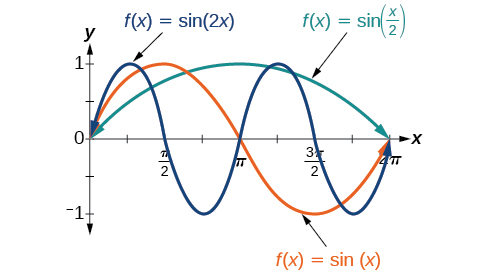
\includegraphics[scale=0.8]{images/sin}
\end{figure}


In the given  \autoref{fig:singraph} the graph of sin x is shown.

\chapter{Here is the Forth Chapter...}

\blindtext 


\section{This is some title of the section}

\blindtext 

\blindtext 



\section{This is some other  title of this section}

\blindtext 

\blindtext 

\chapter{Summary and Future Scope}

\blindtext 


\begin{appendices}
\chapter{Implementation Details}

\blindtext 

\end{appendices}

\fancyhead{}
\fancyhead[R]{\nouppercase\leftmark}

\printbibliography[title={References}]

\clearpage 
\sectionmark{\emph{Subject Index}}
%\addcontentsline{toc}{chapter}{Subject Index}
\printindex

\end{document}